\documentclass{article}
\usepackage{amsfonts}
\usepackage{amsmath}
\usepackage{amssymb}
\usepackage{color}
%\usepackage{apacite}
\usepackage{caption}
\usepackage{graphicx}
\usepackage{algorithm}
\usepackage[noend]{algpseudocode}
\usepackage{adjustbox}
\begin{document}

\author{
  Jonsson, Haukur\\
  \texttt{11137304}
  \and
  Rajamanickam, Santhosh\\
  \texttt{11650702}
  \and
  Rapp, Max\\
  \texttt{11404310}
}
\title{A Qualitative Reasoning Model of a simple (?) Container System\\
	\large Project Report}
\maketitle



\section{Introduction}

Everyday life requires engaging with countless systems of varying complexity. Successful engagement necessitates robust approximate prediction of their behaviour. However, understanding the dynamics of even the simplest of these systems would require solving a set of differential equations of prohibitive complexity.

Rather than precise modelling, humans therefore engage in \textit{Qualitative Reasoning} to understand and predict the behaviour of systems surrounding them. Qualitative models are built by using simplifying \textit{assumptions} to construct a simplified ontology of the system including its objects and the causal relations between them as well as discretizing the quantities of the objects and the magnitudes of the relations. Such models are surprisingly powerful in predicting possible system outcomes.

It is therefore arguable that understanding a domain is a function of one's qualitative model of that domain. In this paradigm, human (and machine) learning and teaching can then be understood in terms of building and adapting qualitative models of the world. 

The computer assisted learning paradigm tries to leverage this approach by developing \textit{Human Level AI} that assists and interacts with the learner in building better qualitative models.

The goal of this project is to implement a qualitative model of a container system that could serve in an interactive learning software by taking various inputs and returning a state graph and trace of the development of the system.

\section{Two Container Models}

The system to be modelled can be described as follows: A \textbf{tap} is used to regulate the influx of water into an open \textbf{container} with a \textbf{drain} through which water escapes.

The basic ingredients needed to build a model for this system are the \textit{entities} which describe the basic objects the model contains. An entity may have one or more \textit{quantities} describing its magnitude. The quantities each have a magnitude constrained by a \textit{quantity space} containing its allowed values as well as a \textit{derivative} with quantity space (-,0,+) describing the current change in quantity. Between quantities \textit{causal relations} obtain. In our case these include \textit{influences} ($I^+$, $I^-$) and \textit{proportionalities} ($P^+$, $P^-$). Influences are positive or negative relationships from the magnitude of a quantity to the derivative of another. Proportionalities are positive or negative relationship from one derivative to another.
Another component we need are \textit{correspondences}. Correspondences can be implications or equivalences between values of quantities' magnitudes.

Using these ingredients, depending on one's assumptions, models of varying complexity of the container system can be devised. Here we describe two. 



\subsection {Model I}

\begin{figure}[!h]
	\centering
	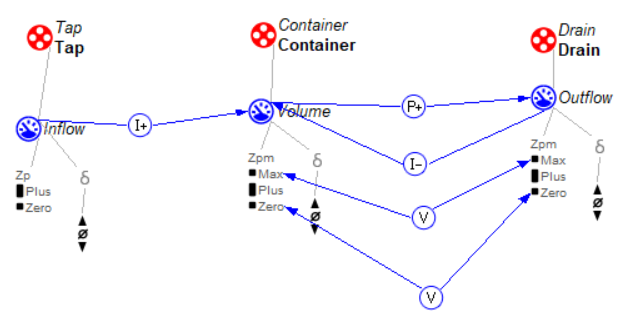
\includegraphics{Simple_Flow.png}
	\caption{Ontology of Model I. Note the red entities which indicate conditions that have to be met for the relations to apply.}
	\label{fig: figure1}
\end{figure}

\textbf{Ontology:}
\begin{itemize}
	\item Entities: Tap, Container, Drain
	\item Quantities(Spaces): Inflow (Zero; Plus), Volume (Zero, Plus, Max), Outflow (Zero, Plus, Max)
	\item Relations: $I^+$(Inflow, Volume), $I^-$(Outflow, Volume), $P^+$(Volume, Outflow)
	\item Correspondences: Volume(Zero)$\leftrightarrow$Outflow(Zero), Volume(Max)$\leftrightarrow$Outflow(Max)
\end{itemize}

The ontology above is depicted in figure \ref{fig: figure1}. To study the development of the system we not only need an ontology but also an \textit{initial state} (or \textit{scenario}). figure \ref{figure2} represents the scenario which we aim to implement for Model I. Namely, we assume that inflow and outflow are at zero in the beginning and that the inflow is exogenously determined by a function taking the form of a positive parabola. I.e. $\delta$Inflow will initially increase but eventually stagnate and start to decrease until it reaches zero.


\begin{figure}[!h]
	\centering
	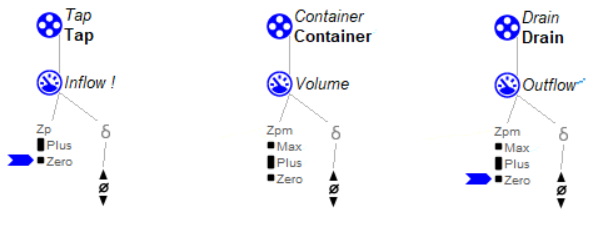
\includegraphics{Scenario_1.png}
	\caption{Initial state of Model I.}
	\label{figure2}
\end{figure}

\subsection {Model II}

\begin{figure}[!h]
	\centering
	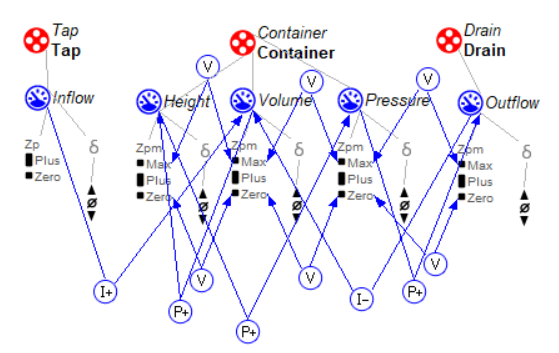
\includegraphics{Extra_Flow.png}
	\caption{In the more complex Model II, outflow is no longer determined by volume but by pressure which is in turn determined by the height of the fluid in the container which is proportional to the volume.}
	\label{figure3}
\end{figure}

\textbf{Ontology:}
\begin{itemize}
	\item Entities: Tap, Container, Drain
	\item Quantities(Spaces): Inflow (Zero; Plus), Height(Zero, Plus, Max), Pressure (Zero, Plus, Max), Volume (Zero, Plus, Max), Outflow (Zero, Plus, Max)
	\item Relations: $I^+$(Inflow, Volume), $I^-$(Outflow, Volume), $P^+$(Volume, Outflow)
\end{itemize}

The more complex ontology of Model II is shown in figure \ref{figure3} and the corresponding initial state (unchanged except for entities) in figure \ref{figure4}.

\begin{figure}[!h]
	\centering
	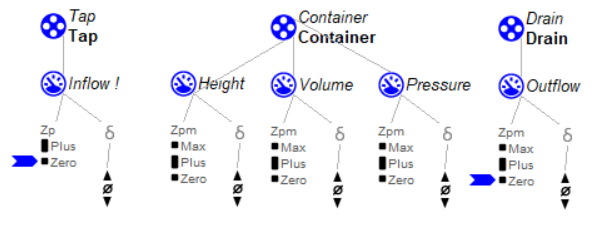
\includegraphics{Scenario_2.png}
	\caption{Initial state of Model II.}
	\label{figure4}
\end{figure}

\section{Target Simulation and State Graph}

To begin with, we set up Model I and Model II in the QR-software \textit{Garp3} to create benchmarks for our implementations. Simulations using default modelling settings (figure \ref{figure5}) lead in both cases to state graphs containing 13 nodes. As expected, the unique end state (state 12 in both cases) consists of an empty container with zero in- and outflow (figure \ref{figure9}). Interestingly, the graphs of the two models look completely identical inspite of the added quantities in Model II (figure \ref{figure7}).


\begin{figure}[!h]
	\makebox[\textwidth][c]{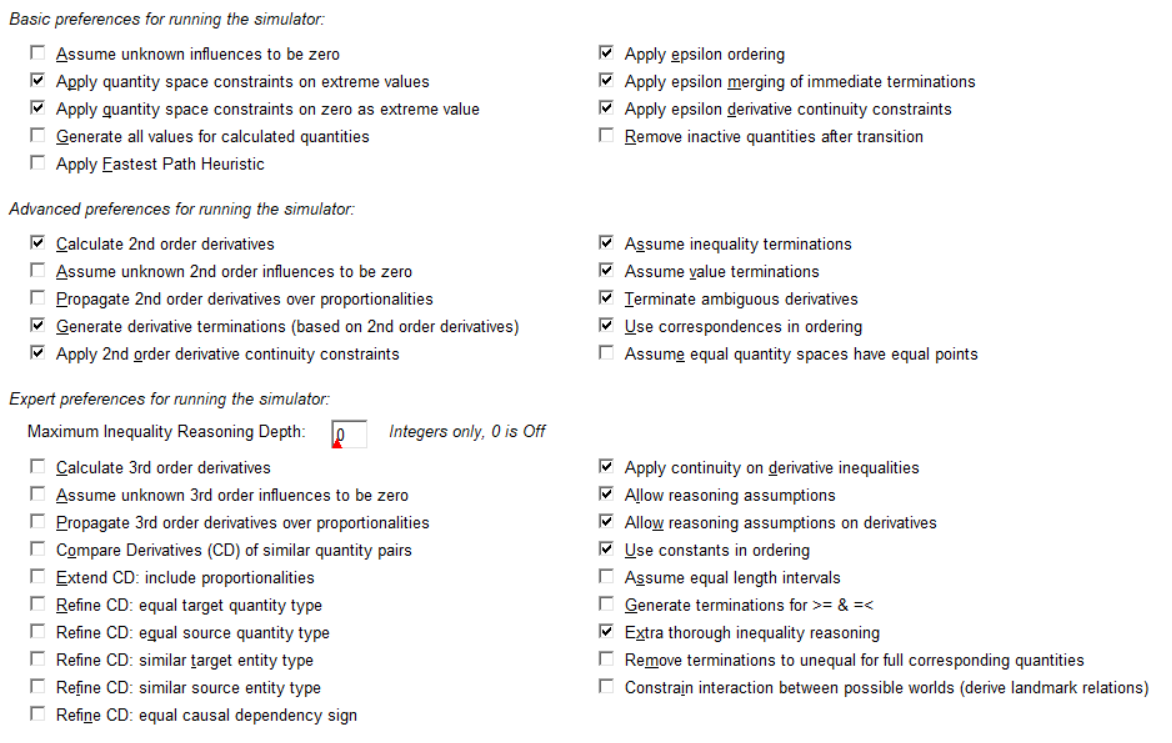
\includegraphics[scale=0.7]{Modelling_Settings}}
	\caption{The modelling preferences used in our benchmark simulations.}
	\label{figure5}
\end{figure}


%\begin{figure}
%	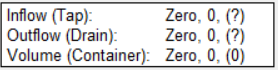
\includegraphics{End_State}
%	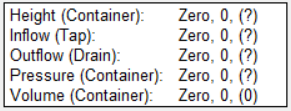
\includegraphics{End_State_Extra}
%	\caption{The end states of the simulations of Model I and II respectively.}
%	\label{figure6}
%\end{figure}

\begin{figure}
	\centering
	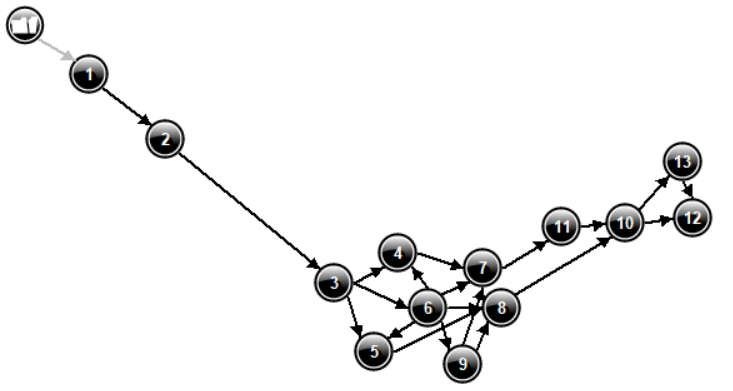
\includegraphics[scale=0.9]{Simple_State_Graph.png}
	\caption{State graph for Model I and II. While the states represented differ in the number of quantities they represent, the identity of the graph representations indicate that Model I and Model II describe the same system in two different yet - with respect to evolution - equivalent ways.}
	\label{figure7}
\end{figure}

\section{Implementation}

\subsection{Environment}

To implement a QR-reasoner for Model I and II we used Python 3.6 including the packages \textit{networkx}, \textit{numpy} and \textit{matplotlib}. To run it use the command line command ``python run\_model.py". Note that uncommenting the graph drawing function may lead to dependency issues. 

\subsection{Modelling Assumptions}

We now set out to recreate the state graphs of Model I and II using a much simpler implementation. Namely, of the simulation preferences described in figure \ref{figure5} we will only implement the following:


\textbf{Basic Epsilon Ordering:} Any termination that consists of a point-value changing to an interval is immediate and takes priority over changes that take time such as interval to landmark changes. If more than one immediate terminations is applicable we apply them in the ordering specified in Algorithm \ref{pointchanges}. In this way we divide the termination calculation into two phases \textit{intra-state changes} and \textit{inter-state changes}. Branching can take place only in the latter phase.

\textbf{Derivative values are point values:} Note that this entails that proportionalities act immediately. This assumption can be justified by the fact that proportionalities are usually the result of having different descriptions of the same state of a system that are pragmatically useful but ontologically reducible to each other. In our case, consider the water column in the container in Model II: the height of the column, its volume and the pressure in the column are three different yet dependent ways of describing the same state of the system; thus if one of these quantities changes, so do the others by definition. Proportionality here thus merely describes the same change by different names and therefore acts immediately.

After inferring terminations, in a third phase, we check the consistency of the termination candidates against the following conditions:

\textbf{No magnitude change without non-zero derivative:} a magnitude of a quantity can only increase/decrease if its derivative is greater/smaller than zero. 

\textbf{No derivative change without (exogenous) influence:} likewise, we don't allow derivative changes that are not caused by an influence, proportionality or exogenous variable. 

\noindent The two preceding conditions immediately imply the next one:

\textbf{No causation by correspondence:} implications and equivalences act as sanity checks and let us throw out inconsistent states but cannot be used in the static/dynamic phases.

\textbf{No fleeting equalities:} If $I^+(A,B)$, $I^-(C,B)$, $A=C$ and $\delta A \neq \delta C$, $\delta B \neq 0$. The justification for this assumption is that such points of fleeting inequality should take priority by epsilon ordering since moving away from a point of equality is immediate. Therefore they should immediately terminate into a different state.

\begin{figure}[!h]
	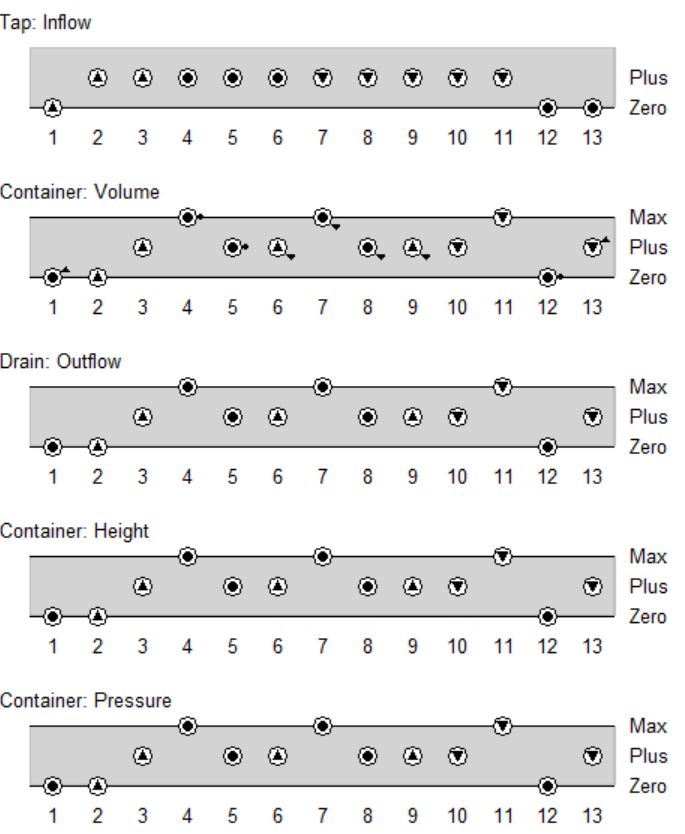
\includegraphics{Value_History_Extra}
	\caption{Value history of Model I \& II (lower part). Notice that state 12 is the end state in both cases.}
	\label{figure9}
\end{figure}

\pagebreak

\subsection{Algorithm}

Note that these assumptions do not touch on issues such as second order derivatives or inequality reasoning. Our algorithm is thus much more primitive than Garp3's. We describe how it works by the following pseudocode:\\\\

\begin{algorithm}[!h]
	\caption{Construct State Graph}\label{stategraph}
	\begin{algorithmic}[1]
		\Procedure{MakeGraph}{intialState,causalGraph}
		\State $\textit{stateGraph} \gets \text{graph.addHead}(\textit{initialState})$
		\State $\textit{stateStack} \gets \text{stack.push}(\textit{initialState})$
		\While {$\text{stack.length(stateStack)} != 0$} 
		\State $\textit{currentState} \gets \text{stack.pop}(stateStack)$
		\State $\textit{nextStates[]} \gets \text{computeNextStates}(currentState,causalGraph)$
		\For {\textit{index} $\gets$ \textit{0} to length(\textit{nextStates})}
		\State $\textit{childState} \gets nextStates[index]$
		\State $\textit{exists} \gets \text{checkStateExists}(state)$
		\If {$\text{not} \textit{exists}$}
		\State assignStateNumber(\textit{childState})
		\State graph.addChild(\textit{stateGraph,currentState,childState})
		\State stack.push(\textit{stateStack,childState})
		\Else 
		\State graph.addChild(\textit{stateGraph,currentState,childState})
		\EndIf
		\EndFor
		\EndWhile
		\State \Return $stateGraph$
		\EndProcedure
	\end{algorithmic}
\end{algorithm}

\textbf{Algorithm 1: makeGraph(initialState,causalGraph)}
\begin{itemize}
	\item This is the method that is used to create the state graph.
	\item It takes the \textit{initialState} and \textit{causalGraph} as parameters.
	\item The \textit{causalGraph} contains information about the entities,  their quantities and the corresponding relationships between them.
	\item The algorithm loops until we get all possible states by computing the possible states that each state can transition to and add them as children to the corresponding state. 
	\item The algorithm also checks whether a state has already been generated previously and if it is already present we just add it as the child to the state from which it transitions from.
\end{itemize}

\begin{algorithm}[!h]
	\caption{Compute next state transitions}\label{nextstate}
	\begin{algorithmic}[1]
		\Procedure{computeNextStates}{currentState,causalGraph}
		\State $newState \gets \text{NULL}$ 
		\State $newState \gets$ applyPointChanges($currentState,causalGraph$)
		\If {newState \text{not NULL}}
		\State $newState \gets$ applyStaticChanges($newState,causalGraph$)
		\State \Return $newState$
		\EndIf
		\State $newStatesList$[ ]
		\State $counter \gets 0$
		\State $newStatesList \gets$ applyIntervalChanges($currentState,causalGraph$)
		\For {$index \gets 0$ to length($nextStatesList$)} 
		\State $newState \gets$ applyStaticChanges($newStatesList[i],causalGraph$)
		\State $isConsistent \gets$ checkStateConsistency($newState$)
		\If {$isConsistent$}
		\State $newStatesList[counter] \gets newState$
		\State counter++
		\EndIf
		\EndFor
		\State \Return $newStatesList$
		\EndProcedure
	\end{algorithmic}
\end{algorithm}
\textbf{Algorithm 2: computeNextState(currentState,causalGraph)}
\begin{itemize}
	\item This is the method that is used to generate the possible state transitions from a single node.
	\item There are three possible updates that can be applied to a state which are: static changes which correspond to intra-state changes as well as point changes and interval changes which correspond to inter-state changes. 
	\item After we get the possible transition states we check whether the states are consistent or not using the function \textit{checkStateConsistency}
\end{itemize}

\begin{algorithm}[!h]
	\caption{Applying Point Changes}\label{pointchanges}
	\begin{algorithmic}[1]
		\Procedure{applyPointChanges}{currentState,causalGraph}
		\State $newState \gets currentState$
		\For {$index1 \gets 0$ to length($causalGraph.entities$)}
		\For {$index2 \gets 0$ to length($causalGraph.entities[index1].quantaties$)}
		\If {$newState[index1][index2].derivavtive == 0$}
		\If {$newState[index1][index2].magnitude == 0$}
		\State applyDerivative($newState[index1][index2]$)
		\EndIf
		\If {$currentState[index1][index2].magnitude == MAX$}
		\State applyDerivative($newState[index1][index2]$)
		\EndIf
		\EndIf
		\EndFor
		\EndFor
		\For {$index1 \gets 0$ to length($causalGraph.relationships$)}
		\If {$causalGraph.relationships[index1] == "Influence"$}
		\State $index2,index3 \gets causalGraph.relationship[index1].recievingPartyIndices$
		\If {$currentState[index2][index3].derivative == 0$}
		\State applyInfluenceRelationship(newState)
		\EndIf
		\EndIf
		\EndFor
		\State \Return $newState$
		\EndProcedure
	\end{algorithmic}
\end{algorithm}

\textbf{Algorithm 3: applyPointChanges(currentState,causalGraph)}
\begin{itemize}
	\item This method applies magnitude changes of the quantities corresponding to its derivatives. 
	\item This method also applies potential influence changes by comparing the derivative of the receiving quantity and the magnitude of the causal quantity.
\end{itemize}

\begin{algorithm}[!h]
	\caption{Applying Static Changes}\label{staticchanges}
	\begin{algorithmic}[1]
		\Procedure{applyStaticChanges}{currentState,causalGraph}
		\State $newState \gets currentState$
		\State $condtion \gets TRUE$
		\While {$condtion == TRUE$}
		\For {$index1 \gets 0$ to length($causalGraph.relationships$)}
		\State $beforeState \gets newState$
		\If {$causalGraph.relationships[index1] == "Proportional"$}
		\State applyProportionalRelationship($newState$)
		\EndIf
		\If {$causalGraph.relationships[index1] == "Equivalence"$}
		\State applyEquivalenceRelationship($newState$)
		\EndIf
		\State $condition \gets ifDifferent(beforeState,newState)$
		\EndFor
		\EndWhile
		\State \Return $newState$
		\EndProcedure
	\end{algorithmic}
\end{algorithm}


\textbf{Algorithm 4: applyStaticChanges(currentState,causalGraph)}
\begin{itemize}
	\item Checks for proportional relationships.
	\item Checks for equivalence relationships.
\end{itemize}

\begin{algorithm}[!h]
	\caption{Applying Interval Changes}\label{intervalchanges}
	\begin{algorithmic}[1]
		\Procedure{applyStaticChanges}{currentState,causalGraph}
		\State $newState \gets currentState$
		\State $newStatesList$[ ]
		\State $counter=0$
		\For {$index1 \gets 0$ to length($causalGraph.relationships$)}
		\If {$causalGraph.relationships[index1] == "Influence"$}
		\State applyInfluenceRelationship(newState)
		\EndIf
		\If {ifDifferent($nextState,currentState$)}
		\State $newStatesList[counter] \gets newState$
		\State $counter++$
		\EndIf
		\EndFor
		\State $newState \gets currentState$
		\For {$index1 \gets 0$ to length($causalGraph.entities$)}
		\For {$index2 \gets 0$ to length($causalGraph.entities[index1].quantaties$)}
		\State applyDerivative($newState[index1][index2]$)
		\If {ifDifferent($nextState,currentState$)}
		\State $newStatesList[counter] \gets newState$
		\State $counter++$
		\EndIf
		\EndFor
		\EndFor
		\State $newState \gets currentState$
		\State $newState \gets$ applyExogenous($causalgraph.typeOfExogenous,newState$)
		\If {ifDifferent($nextState,currentState$)}
		\State $newStatesList[counter] \gets newState$
		\State $counter++$
		\EndIf
		\State \Return $newStatesList$
		\EndProcedure
	\end{algorithmic}
\end{algorithm}

\textbf{Algorithm 5: applyIntervalChanges(currentState,causalGraph)}
\begin{itemize}
	\item This method indicates the changes that can happen over a time interval.
	\item This method applies the influence relationship and derivative changes and records all possible state transitions from the \textit{currentState}
	\item This method also applies exogenous change corresponding to the type of exogenous function in the \textit{causalGraph} by updating the derivative of the inflow.  
\end{itemize}

\section{Results}

Which deviations from the benchmark simulations will our modelling choices incur? And do they affect the overall degree to which our algorithm captures the behaviour of the system? 

The results of our simulations are visualized by the state graph in figure \ref{figure8} as well as the state descriptions in table \ref{table1}. Consistently with the Garp3 simulations we found that the state graphs of Model I and Model II coincide. Our algorithm also resulted in the same end state as the Garp3 implementation, showing that it captured the overall system behaviour well.

However, given the comparative simplicity of our algorithm, comparing our results with the benchmarks yields the following divergences:

\begin{itemize}
	\item \textbf{States 9 and 10-17:} Here $\delta$ Inflow is negative although the inflow has already reached tero. This is excluded by the Garp3 modelling assumption ``Apply quantity space constraints on zero as extreme Value" which we did not implement. However, it has no effects in this model.
	\item \textbf{States 11-13:} These states do not appear in the Garp3 state graph. The reason is that state 11 is spurious: we have zero inflow and yet maximum volume and positive $\delta$ Volume. This happens since our algorithm does not check for second round effects of influence changes: when Inflow goes to zero this has the immediate second round effect of its influence on $\delta$ Volume becoming 0 thus being outweighed by $I^-$(Outflow, Volume) chaning $\delta$ Volume to 0 (third round effects abound). Instead, our algorithm only applies these second and third round effects step by step in states 12-14 which deterministically follow from 11. 
	\item  \textbf{State 15:} The same holds for state 15. Note that state 13 in figure \ref{figure9} has a positve $\delta^2$ Volume. This indicates the possibility to go to an equivalent to state 15 of our algorithm. However, this state is inconsistent to Garp3 since the immediate second round effect of $I^-$(Outflow, Volume) prevents transition to this state. Again, this is instead done step by step in two states by our algorithm.
	\item \textbf{State 16:} For the same reason, the algorithm takes two steps to transition from state 15 to state 17 resulting in the intermediary state 16
\end{itemize}



\begin{figure}
	\centering
	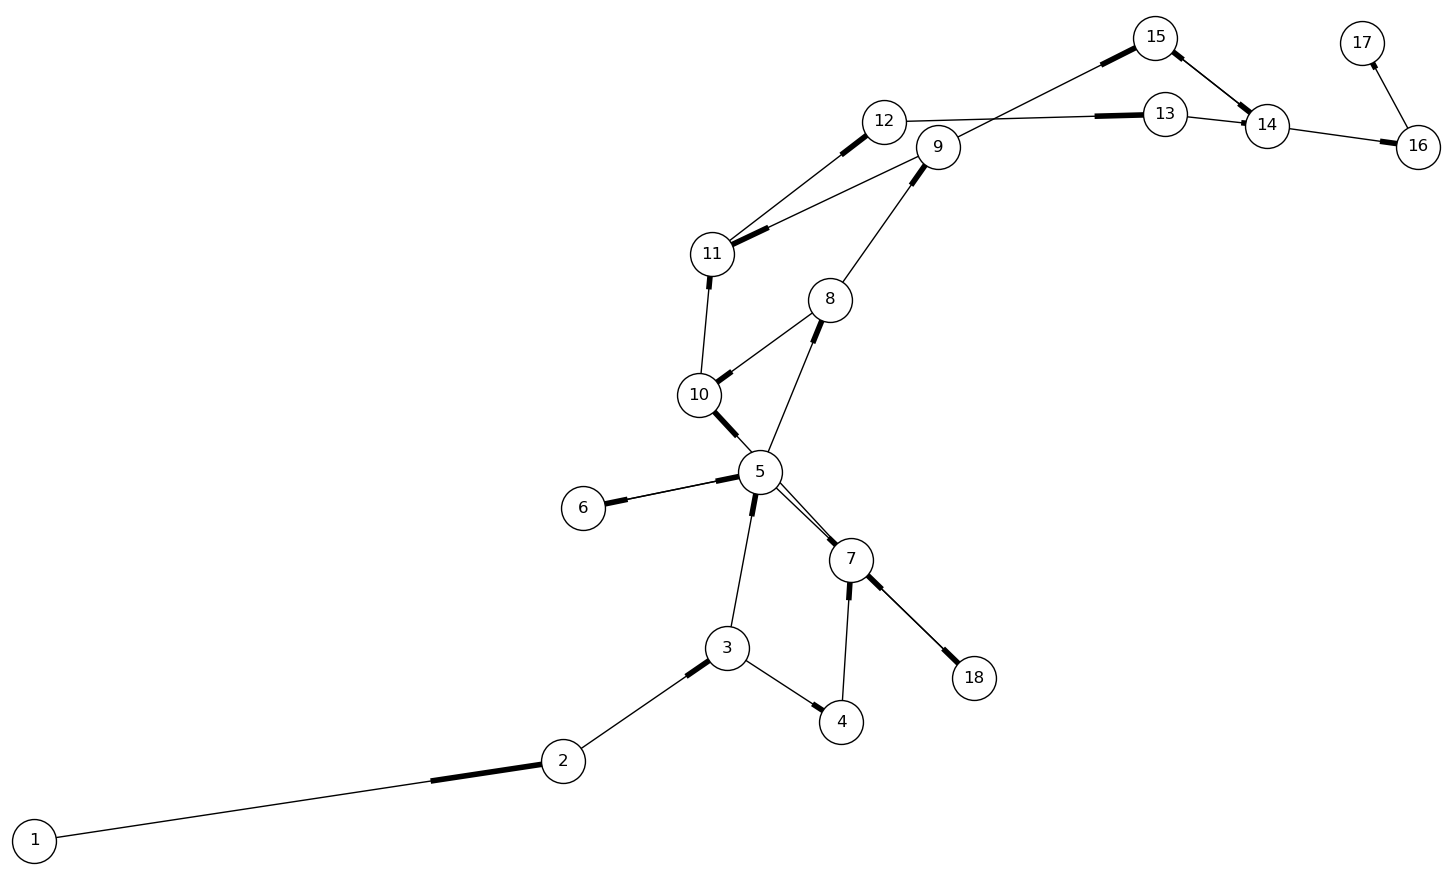
\includegraphics[scale=0.3]{Ok_State_Graph.png}
	\caption{State graph for Model I and II according to our simulation. }
	\label{figure8}
\end{figure}

%\begin{table}[]
	%\centering
	%\caption{State table of Model I}
	%\label{table1}
	%\begin{tabular}{llllllll}
		%#  & Inflow & $\delta$ Inflow & Volume & $\delta$ Volume & Outflow %& $\delta$ Outflow & Children \\
		%1  & 0      & +               & 0      & 0               & 0       %& 0                & 2        \\
		%2  & +      & +               & 0      & +               & 0       %& +                & 3        \\
		%3  & +      & +               & +      & +               & +       %& +                & 4, 5     \\
		%4  & +      & +               & Max    & +               & Max     %& +                & 7        \\
		%5  & +      & 0               & +      & +               & +       %& +                & 6, 7, 8  \\
		%6  & +      & 0               & +      & 0               & +       %& 0                & 5        \\
		%7  & +      & 0               & Max    & +               & Max     %& +                & 10, 18   \\
		%8  & +      & -               & +      & +               & +       %& +                & 9, 10    \\
		%9  & 0      & -               & +      & +               & +       %& +                & 11, 15   \\
		%10 & +      & -               & Max    & +               & Max     %& +                & 11       \\
		%11 & 0      & -               & Max    & +               & Max     %& +                & 12       \\
		%12 & 0      & -               & Max    & 0               & Max     %& 0                & 13       \\
		%13 & 0      & -               & Max    & -               & Max     & -                & 14       \\
		%14 & 0      & -               & +      & -               & +       & -                & 15, 16   \\
		%15 & 0      & -               & +      & 0               & +       & 0                & 14       \\
		%16 & 0      & -               & 0      & -               & 0       & -                & 17       \\
		%17 & 0      & -               & 0      & 0               & 0       & 0                & End      \\
		%18 & +      & 0               & Max    & 0               & Max     & 0                & 7       
	%\end{tabular}
%\end{table}


\begin{table}
	\small
	\begin{adjustbox}{center}
	\begin{tabular}{@{}llllllllllll}
		\# & Inflow & $\delta$ Inflow & Volume & $\delta$ Volume & Outflow & $\delta$ Outflow & Children & Height & $\delta$ Height & Pressure & $\delta$ Pressure  \\
		1  & 0      & +           & 0      & 0           & 0       & 0            & 2        & 0      & 0                                & 0        & 0                                   \\
		2  & +      & +           & 0      & +           & 0       & +            & 3        & 0      & +                                & 0        & +                                   \\
		3  & +      & +           & +      & +           & +       & +            & 4, 5     & +      & +                                & +        & +                                   \\
		4  & +      & +           & Max    & +           & Max     & +            & 7        & Max    & +                                & Max      & +                                   \\
		5  & +      & 0           & +      & +           & +       & +            & 6, 7, 8  & +      & +                                & +        & +                                   \\
		6  & +      & 0           & +      & 0           & +       & 0            & 5        & +      & 0                                & +        & 0                                   \\
		7  & +      & 0           & Max    & +           & Max     & +            & 10, 18   & Max    & +                                & Max      & +                                   \\
		8  & +      & -           & +      & +           & +       & +            & 9, 10    & +      & +                                & +        & +                                   \\
		9  & 0      & -           & +      & +           & +       & +            & 11, 15   & +      & +                                & +        & +                                   \\
		10 & +      & -           & Max    & +           & Max     & +            & 11       & Max    & +                                & Max      & +                                   \\
		11 & 0      & -           & Max    & +           & Max     & +            & 12       & Max    & +                                & Max      & +                                   \\
		12 & 0      & -           & Max    & 0           & Max     & 0            & 13       & Max    & 0                                & Max      & 0                                   \\
		13 & 0      & -           & Max    & -           & Max     & -            & 14       & Max    & -                                & Max      & -                                   \\
		14 & 0      & -           & +      & -           & +       & -            & 15, 16   & +      & -                                & +        & -                                   \\
		15 & 0      & -           & +      & 0           & +       & 0            & 14       & +      & 0                                & +        & 0                                   \\
		16 & 0      & -           & 0      & -           & 0       & -            & 17       & 0      & 0                                & 0        & 0                                   \\
		17 & 0      & -           & 0      & 0           & 0       & 0            & End      & 0      & 0                                & 0        & 0                                   \\
		18 & +      & 0           & Max    & 0           & Max     & 0            & 7        & Max    & 0                                & Max      & 0                                  
	\end{tabular}
	\end{adjustbox}
	\caption{State table of Model I \& II (right of children)}
	\label{table1}
\end{table}

\section{Conclusions}

In this project we implemented two models of a simple container system. Using a qualitative reasoning algorithm we explored the time evolution of these models. We found that our algorithm's state graph was well in line with intuition as well as with simulations of more advanced QR-software. In future implementations we would use an event based approach to deal with the immediate termination of second and third round effects. 

\end{document}